\section{Software Development Lifecycle}

\begin{figure}[!htp]
    \centering
    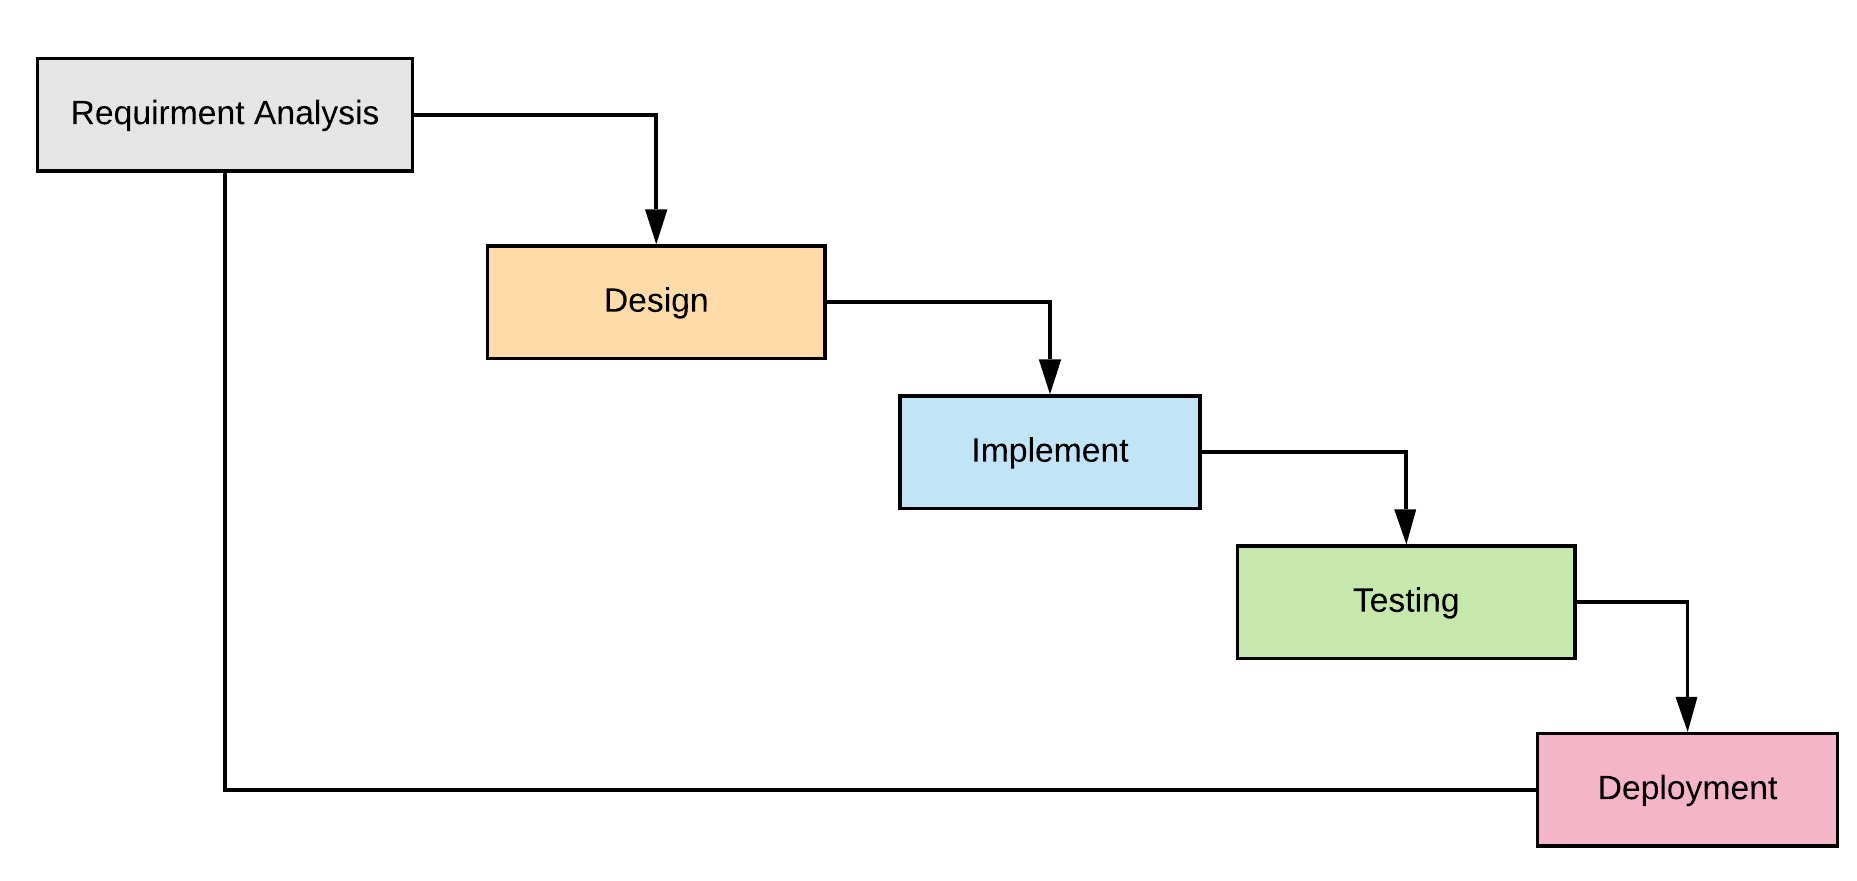
\includegraphics[width=.8\textwidth]{Images/waterfall}
    \caption{Waterfall Model}
    \label{fig:waterfall}
\end{figure}


The waterfall software development lifecycle was used during developing the project. The waterfall
model also known as linear-sequential life cycle model focuses on completing each phase of
development before switching to the next stage of development Cite{1}. The waterfall model was
accurate for this project as the scope of the project is small and was developed individually. Output
from each phase of development lifecycle acts as the input to the next phase. The figure above
\ref{fig:waterfall} shows the various phases of the waterfall development lifecycle. In initial phase of the
development the requirements and targeted audience were analysed as mentioned in the
introduction section of the project. The second phase involved developing conceptual models using
UML(Unified Modelling Language) to design the system using component diagram which captures
the structural and sequence diagram to capture the behavioural design of the system. The next
phase of waterfall model was implementation of the intelligent system to detect pigmented skin
lesions. The implementation phase of the lifecycle involved developing convolutional network and
performing various experiments to get optimal performance. Furthermore, The next phase of
development was to test the effectiveness of the overall system for which the prediction results
gathered from medical professionals in the form of questionnaires were compared with the
automated system and results were analysed with confusion matrix. The last phase was to deploy
the model to the web-based system which was done by converting the keras model to json file and
using tensorflowjs. At last, the maintenance phase of lifecycle cannot be applied to short term
project.

\pagebreak
\section{Work Managment System}
\begin{figure}[!htp]
    \centering
    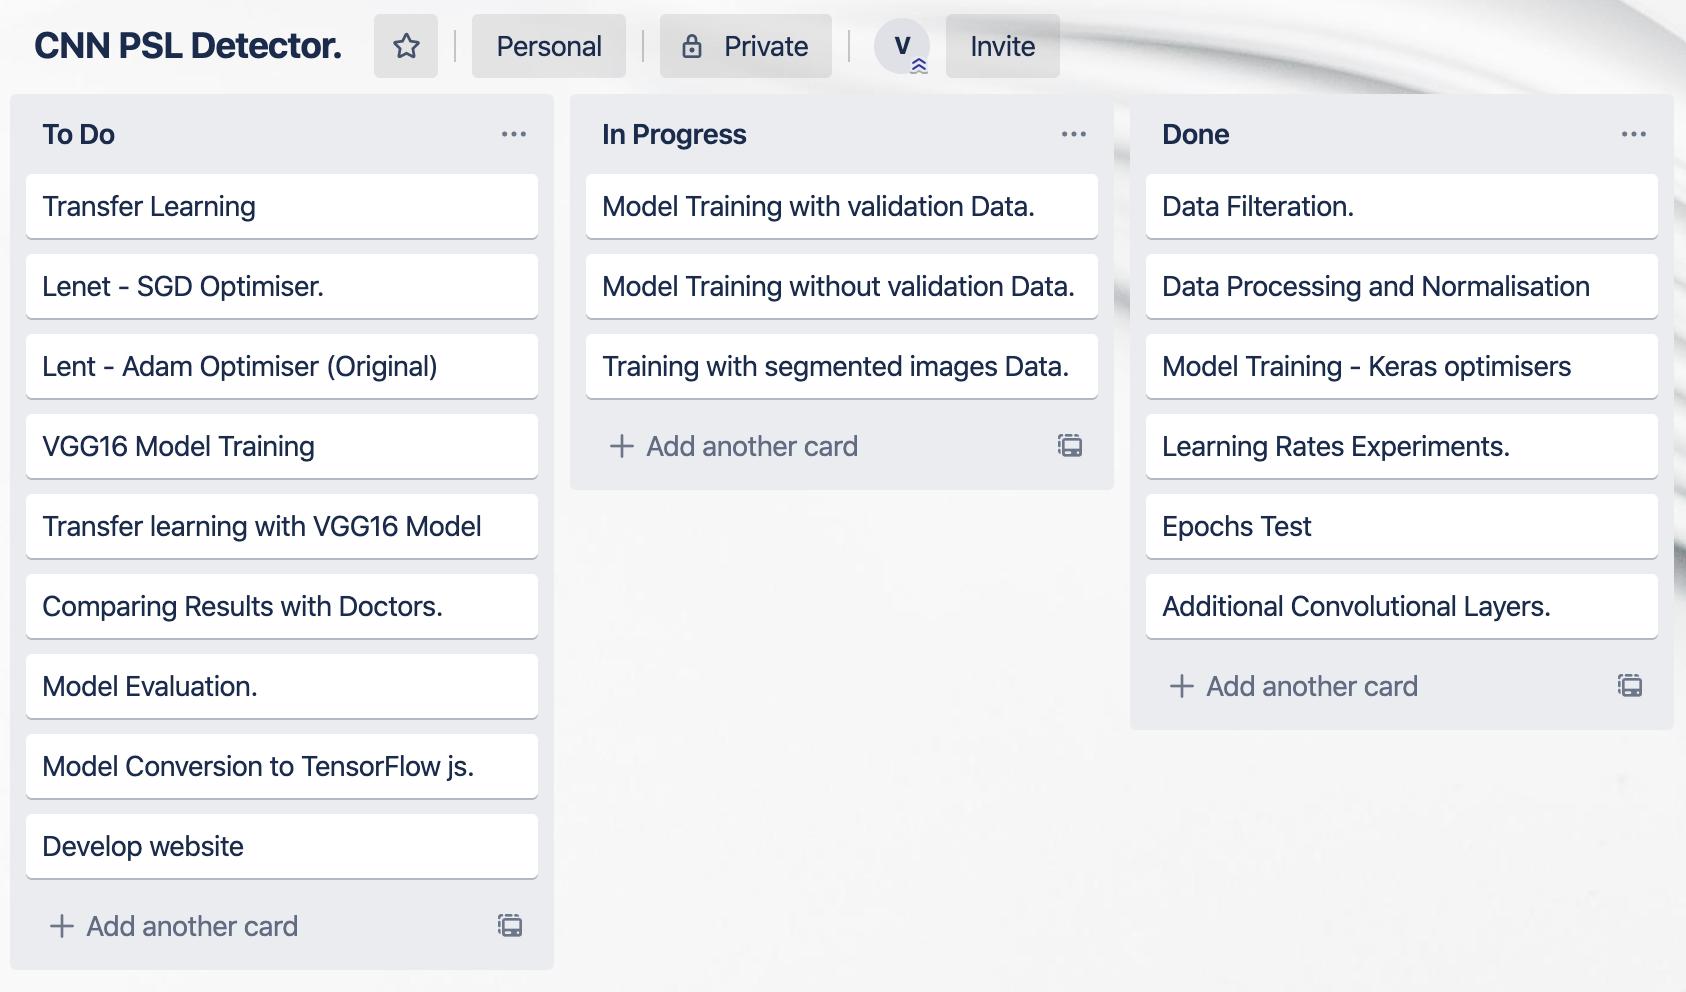
\includegraphics[width=15cm]{Images/Kanban Bords.png}
    \caption{Kanban Board}
\end{figure}
\pagebreak
\section{Version Control}



